\chapter{LITERATURE REVIEW}
\label{chap-two}
Bridges are designed based on discrete events assuming that the initial material and structure properties remain constant through the life of the bridge. The purpose of the research described is to study condition dependent performance based design that considers the material and geometric properties as the structure ages, as well as the effects of multiple and discrete events on the achievement of prescribed limit states.

In this chapter, the available knowledge on the different topics that are available in the literature are synthesized. First, a review on the different definitions of commutative damage is presented then the main idea for this research is established and its required components.

\section{Cumulative Damage}

There have been attempts by many researchers to establish the best way to account for the accumulation of damage. The measures are described in this section.

\subsection{Damage Index}
The effect of cumulative damage in structures was studied by Park and Ang (1985) \cite{Young-JiPark1985} in their study the authors proposed the damage index as shown in \ref{eq.DamageIndex}. The damage index was used as a measure to quantify damage in terms of the maximum experienced earthquake and the absorbed hysteretic energy.

\begin{equation}
  D=\frac{\Delta_{m}}{\Delta_{u}}-\beta \frac{E_h}{F_{y}\Delta{u}}
  \label{eq.DamageIndex}
\end{equation} 

$\Delta_{m}$: Maximum deformation under earthquake

$\Delta_{u}$: Ultimate deformation under monotonic loading

$F_{y}$: Calculated yield strength

$E_{h}$: Total hysteretic energy

$\beta$: Dimensionless constant 

\begin{figure}[htbp]
\centering
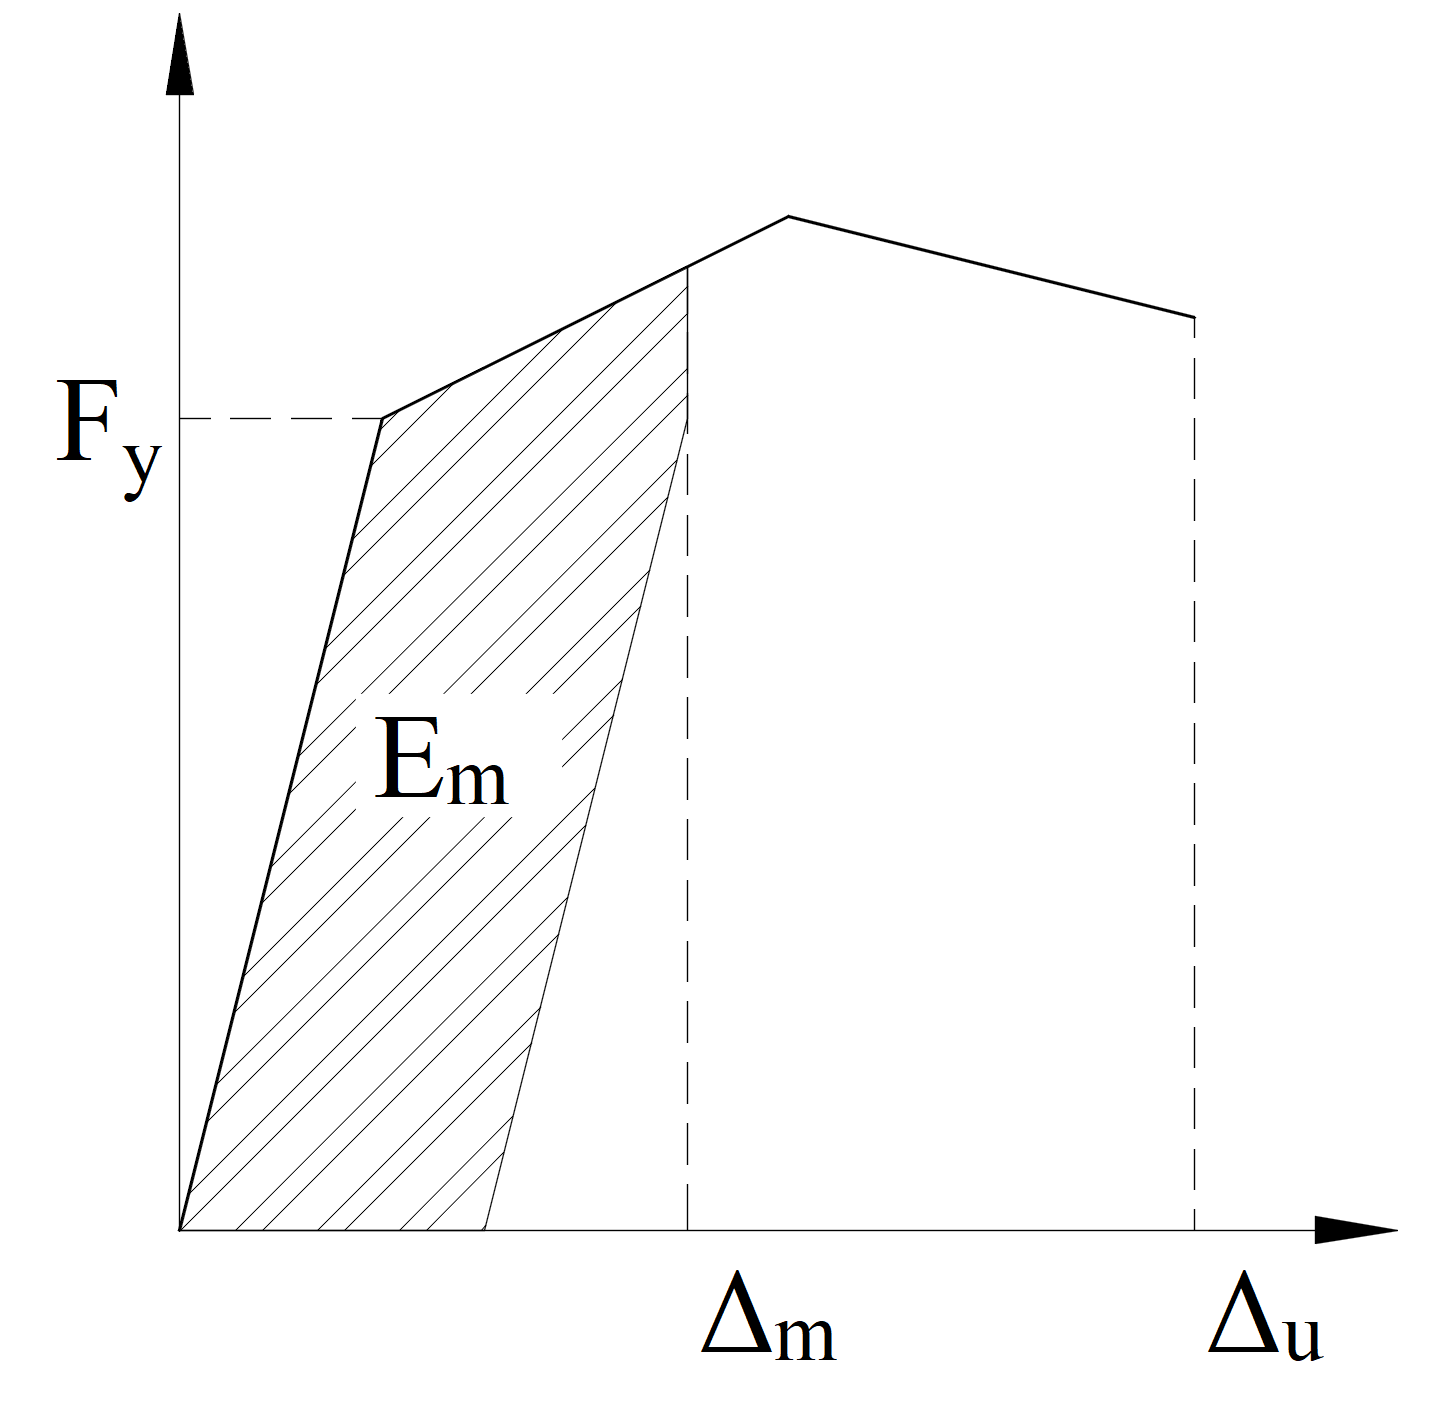
\includegraphics[width=0.6\textwidth]{Chapter-2/figs/Park_and_Ang_Model}
\caption{Park and Ang conceptual scheme}
\label{fig:Paa}
\end{figure}

Equation \ref{eq.DamageIndex} was derived for concrete elements. The first term here is a simple, pseudo-static displacement measure. The second term accounts for cumulative damage. A figure on the concept is shown in \fref{fig:Paa}. The advantages of this model are its simplicity and flexibility in adapting the model to correlate with experimental data.  

This model has several limitations. Firstly the calibration of the $\beta$ coefficient with observed damage has shown to be very low ($\beta=0.05-0.15$) \cite{Young-JiPark1985} \cite{Ghosh2015}, rendering the second term relatively inconsequential compared to the contribution of the first term. A sample result is taken from Gosh et al \cite{Ghosh2015}, which applied a modified version of the Park and Ang damage index in terms of the moment ($M_{y}$), the rotation ($\theta_y$), and curvature ductility ($\mu$) the modified model is expressed in equation \eref{eq.DamageIndexGhosh}.

\begin{equation}
	D=\frac{\mu_{m}}{\mu_{u}}-\beta\frac{E_h}{M_{y}\theta_y\mu{u}}
	\label{eq.DamageIndexGhosh}
\end{equation}

Using the following values: $\mu_{m}=4.93$; $\mu_{u}=17.02$; $M_{y}=8751.375$; $\theta_y=0.0042$; $E_{h}=119.07$; $\beta=0.05$ 

And substituting in equation \eref{eq.DamageIndexGhosh}:
\[
 D=\frac{\mu_{m}}{\mu_{u}}-\beta\frac{E_h}{M_{y}\theta_y\mu{u}}=0.3
	\]
\textbf{First term}:
\[
\frac{\mu_{m}}{\mu_{u}}=\frac{4.93}{17.02}=0.2897
\]
\textbf{Second term}: 
\[	
	\beta \frac{E_h}{M_{y}\theta_y\mu{u}}=0.05\frac{119.07}{8751.375*0.0042*17.02}=0.0103
\]

It can be seen that 97\% of the damage index comes from the first term which is the elastic term and the inelastic part is only 3\% of the total. In addition, the model was derived for reinforced concrete with poor shear detailing. 

Depite its limitation, several studies have used or modified this model to study the effects of cumulative damage for different structures,  of relevant importance are those performed by \cite{Kunnath1992}, who used a modified Park and Ang model, to model damagae at the local level for elements in a structural analysis program IDARC 3.0, in this software for the case of multiple degrees of freedom buildings they also added parameters to consider the damage at the inter-story level and the global model. Ghosh et al \cite{Ghosh2015} developed a damage accumulation framework to develop probabilistic estimates of exceeding a damage index for multiple ground motions. Other regressions have been proposed by \cite{Khashaee}, \cite{Fajfar1992}, \cite{Roufaiel} but show no improvement in assessing the damage state of a structure. While these studies provide an insight into some of the characteristics of damage accumulation they rely on the Park and Ang model and therefore carry the same limitations.

Krawinkler (1987) \cite{Krawinkler1987} proposed a method that considered damage as a function of low cycle fatigue parameters, the form of the Krawinkler damage index for steel components, weldments, and local buckling has a general shape of the Miner model. This model relies on the accumulation of plastic deformations. While this model has proven to work well for the evaluation of individual steel structure elements, it does not provide a way to generalize damage for other types of structures.

\subsection{Probabilistic Approach}

In recent years studies have focused on the effect of cumulative damage. These studies have focused on assessing the damage accumulation under different loading conditions such as multiple earthquakes, corrosion and life span of the structure. Two main approaches to tackle this field of study have been observed:

\begin{itemize}
	\item Probabilistic framework
	\item Fragility curves
\end{itemize}

\textbf{Proababilistic Framework}

One of the most widely used probabilistic framework is the Pacific Earthquake Engineering Research Center (PEER) Performance Based Design. PEER PBD can be expressed by the following equation:
\begin{equation}
\nu_{DM}(dm^{LS})=\iint D_{DM|EDP}(dm|edp)|,dG_{EDP|IM}(edp|im)||\,d\nu_{IM}(im)|
\end{equation}

Mackie et al \cite{Mackie2007} on the basis of the PEER PBD developed the performance based damage design (PBDD) and performance based loss design (PBLD) by defining the probabilistic demand, damage, and loss model parameters in terms of reinforced concrete column damage. The RC column damage was defined in terms of drift ratios defined for the limit states of concrete spalling, bar buckling and failure. 

The authors show that for a given intensity measure (IM) and a confidence level of achieving a limit state, its is possible then to define the probability  of exceeding that limit state.

While this methodology was able to define damage and incorporate it into the PEER PBD framework, the authors did not consider  strain to define the limit states. Also recent research has shown that other intensity measures such as spectral displacement at effective first mode period ($S_{d}(T_{1})$) provide a better intensity measure \cite{Krish2018}.

\textbf{Fragility Curves}

Another common trend in this subject is the use of fragility curves to estimate the effect of damage in structures. Two main approaches were found in the literature. One of them relied on the Park and Ang Model damage index to define damage. While the second approach relates damage to drift.

Ghosh et al \cite{Ghosh2015} formulated a damage accumulation framework. Their study relied on the Park and Ang Damage index explained in the previous section. The study performed a series of nonlinear time history analyses for two cases:

\begin{itemize}
	\item Using a constant main shock hazard occurrence rate (3 main shocks in a 50 year period)
	\item Mainshock - Aftershock series using time-dependent aftershock hazard occurrence rate
\end{itemize}

Evaluation of the damage index exceeding probability for the two cases was performed. The results from this study show regression equations that statistically predict the damage index as a function of earthquake intensity and damage history. This study revealed that for both mainshock and aftershock scenarios there was a significant increase in the probability of damage index exceedance under repeated shock scenarios. While this study shows the importance of considering damage accumulation, these results have to be taken with caution since it carries the same disadvantages of the Park and Ang damage index.

Ghosh et al \cite{Ghosh2010} also studied the effects of corrosion in time dependent seismic fragility curves. Their study characterizes corrosion in concrete columns as a continuous phenomenon that occurs as a function of time. Additionally, the authors considered the effects of corrosion in steel bridge bearings. The authors then ran a series of NLTHA analyses for different aging times of the structures. Based on their analysis time dependent fragility curves were presented. The results showed that as time increases, and as a consequence corrosion increases, the probability of exceeding a limit state increases. In this study limit states where defined on the basis of inter-story drifts which were obtained from experimental results and field observations \cite{Padgett2007}. It is important to mention that the limit states used in their study, were not defined on the basis of strains or other structural property rather from a survey performed in central southeastern United States departments of transportation on the premise of a range of experienced inter-story drifts and the time to repair them. Additionally assuming that corrosion is a continuous process has to be cautiously taken as valid since site information such as temperature, water to cement ratio, the addition of cementitious materials such as silica fume, and the environment (e.g. coastal vs inland) affect the rate of propagation of corrosion\cite{Thoft-Christensen}.

While these studies provide a general view on how damage increases the likelihood of observing collapse or deterioration of the seismic performance, the methods used to arrive at those conclusions can be misleading since the definition of damage as either a Damage Index or Drift are not the best parameters to quantify the damage. It is our belief that strain-based limit states will provide a better understanding on the implications of damage accumulation.
